\section{Derivation of the loss function} \label{derivation_adaptive_loss}
One of the characteristics of orbitals is that they are orthonormal to each other. But if we try to fit orbitals naively we won't be able to guarantee this property. To ensure that the fitted orbitals are orthonormal we can use the following loss function wich enforces the orthogonormality of the orbitals using laplace multipliers:
\begin{align}
    \{\phi_i\}_{i=1,...,N_e} = \underset{\{\phi_i\}_{i=1,...,N_e} pairwise orthonormal}{\text{argmin}}\sum\limits_{i=1}^{N_e} \int (\phi_i(\mathbf{r})-\phi'_i(\mathbf{r}))^2 d\mathbf{r}
\end{align}
In components we can define the lagrangian as:
\begin{align}
\mathcal{L}(\{C_{i\mu}\}_{i=1,...,N_e,\mu=1,...,N_b}) &= \sum\limits_{i=1}^{N_e} \int (\phi_i(C,\mathbf{r})-\phi'_i(\mathbf{r}))^2 d\mathbf{r} + \sum\limits_{i=1}^{N_e} \sum\limits_{j=1}^{N_e} \lambda_{ij}\left( \int \phi_i(C,\mathbf{r})\phi_j(C,\mathbf{r}) d\mathbf{r}- \delta_{ij}\right)\\
    &= \sum\limits_{i=1}^{N_e} C_{i,\mu} \langle \eta_\mu|\eta_\nu \rangle C_{i,\nu} - 2 C_{i,\mu} \langle \eta_\mu|\eta'_\nu \rangle C'_{i,\nu} + C'_{i,\mu} \langle \eta'_\mu|\eta'_\nu \rangle C'_{i,\nu}\\
    &+ \sum\limits_{i=1}^{N_e} \sum\limits_{j=1}^{N_e} \lambda_{ij}\left( C_{i,\mu} \langle \eta_\mu|\eta_\nu \rangle  C_{j,\nu} - \delta_{ij}\right)
\end{align}
Where $\{\lambda_{ij}\}_{i,j=1,...,N_e}$ are lagrange multipliers.
We can now differentiate the lagrangian with respect to the coefficients $C_{i,\mu}$ to get the following equation:
\begin{align}
    \partial_{C_{k,\gamma}}\mathcal{L} &= 2\langle \eta_\gamma|\eta_\nu \rangle C_{k,\nu} - 2 \langle \eta_\gamma|\eta'_\nu \rangle C'_{k,\nu} + 2 \sum\limits_{j=1}^{N_e} \lambda_{kj} \langle \eta_\gamma|\eta_\nu \rangle  C_{j,\nu} = 0\label{deriv_eq}\\
    \partial_{\lambda_{ij}}\mathcal{L} &= C_{i,\mu} \langle \eta_\mu|\eta_\nu \rangle  C_{j,\nu} - \delta_{ij} = 0
\end{align}
Now we contract it with $C_{l,\gamma}$ and $C'_{l,\mu} \langle \eta'_\mu|\eta_\sigma \rangle\langle \eta_\cdot|\eta_\cdot \rangle^{-1}_{\sigma\gamma}$:
\begin{align}
    C_{l,\gamma}\partial_{C_{k,\gamma}}\mathcal{L} &= 2 C_{l,\gamma}\langle \eta_\gamma|\eta_\nu \rangle C_{k,\nu} - 2 C_{l,\gamma} \langle \eta_\gamma|\eta'_\nu \rangle C'_{k,\nu} + 2 \sum\limits_{j=1}^{N_e} \lambda_{kj} C_{l,\gamma}  \langle \eta_\gamma|\eta_\nu \rangle  C_{j,\nu} \\
    &= 2 \delta_{lk} - 2 C_{l,\gamma} \langle \eta_\gamma|\eta'_\nu \rangle C'_{k,\nu} + 2 \sum\limits_{j=1}^{N_e} \lambda_{kj} \delta_{lj}\\
    &=2 \delta_{lk} - 2 C_{l,\gamma} \langle \eta_\gamma|\eta'_\nu \rangle C'_{k,\nu} + 2 \lambda_{kl}= 0\\
        &\Rightarrow C_{l,\gamma} \langle \eta_\gamma|\eta'_\nu \rangle C'_{k,\nu} = \delta_{lk} + \lambda_{kl}\label{xyz}\\
    C'_{l,\mu} \langle \eta'_\mu|\eta_\sigma \rangle\langle \eta_\cdot|\eta_\cdot \rangle^{-1}_{\sigma\gamma}\partial_{C_{k,\gamma}}\mathcal{L} &= 2 C'_{l,\mu} \langle \eta'_\mu|\eta_\sigma \rangle\langle \eta_\cdot|\eta_\cdot \rangle^{-1}_{\sigma\gamma}\langle \eta_\gamma|\eta_\nu \rangle C_{k,\nu} - 2 C'_{l,\mu} \langle \eta'_\mu|\eta_\sigma \rangle\langle \eta_\cdot|\eta_\cdot \rangle^{-1}_{\sigma\gamma} \langle \eta_\gamma|\eta'_\nu \rangle C'_{k,\nu}\\
    &+ 2 \sum\limits_{j=1}^{N_e} \lambda_{kj} C'_{l,\mu} \langle \eta'_\mu|\eta_\sigma \rangle\langle \eta_\cdot|\eta_\cdot \rangle^{-1}_{\sigma\gamma} \langle \eta_\gamma|\eta_\nu \rangle  C_{j,\nu} \\
    &=2 C'_{l,\mu} \langle \eta'_\mu|\eta_\nu \rangle C_{k,\nu} - 2 C'_{l,\mu} \langle \eta'_\mu|\eta_\sigma \rangle\langle \eta_\cdot|\eta_\cdot \rangle^{-1}_{\sigma\gamma} \langle \eta_\gamma|\eta'_\nu \rangle C'_{k,\nu}\\
    &+ 2 \sum\limits_{j=1}^{N_e} \lambda_{kj} C'_{l,\mu} \langle \eta'_\mu|\eta_\nu \rangle  C_{j,\nu} =0\label{last}
    \end{align}
Now insert \eqref{xyz} into \eqref{last}:
\begin{align}
    0&=\delta_{lk} + \lambda_{kl} - C'_{l,\mu} \langle \eta'_\mu|\eta_\sigma \rangle\langle \eta_\cdot|\eta_\cdot \rangle^{-1}_{\sigma\gamma} \langle \eta_\gamma|\eta'_\nu \rangle C'_{k,\nu} + \sum\limits_{j=1}^{N_e} \lambda_{kj} \left(\delta_{lj} + \lambda_{lj}\right) \\
    &= \sum\limits_{j=1}^{N_e} \lambda_{kj}\lambda_{jl} +2\lambda_{kl} - C'_{l,\mu} \langle \eta'_\mu|\eta_\sigma \rangle\langle \eta_\cdot|\eta_\cdot \rangle^{-1}_{\sigma\gamma} \langle \eta_\gamma|\eta'_\nu \rangle C'_{k,\nu} + \delta_{lk}
\end{align}
This is just a quadratic matrix equation which can be solved for $\lambda_{kl}$.\\
We now define
\begin{equation}
    A_{ij}:= C'_{i,\mu} \langle \eta'_\mu|\eta_\sigma \rangle\langle \eta_\cdot|\eta_\cdot \rangle^{-1}_{\sigma\gamma} \langle \eta_\gamma|\eta'_\nu \rangle C'_{j,\nu}
\end{equation}
\begin{align}
    \lambda_{lk,\pm} = \delta_{lk} \pm \sqrt{\delta_{lk}+A_{lk}-\delta_{lk}} = \delta_{lk} \pm \sqrt{A_{lk}}
\end{align}
Now we can insert the lagrange multipliers back into \eqref{deriv_eq} and invert it:
\begin{align}
   0&=\langle \eta_\gamma|\eta_\nu \rangle C_{k,\nu} - \langle \eta_\gamma|\eta'_\nu \rangle C'_{k,\nu} + \sum\limits_{j=1}^{N_e} \left(\delta_{kj} \pm \sqrt{A_{kj}}\right) \langle \eta_\gamma|\eta_\nu \rangle  C_{j,\nu}\\
    &= - \langle \eta_\gamma|\eta'_\nu \rangle C'_{k,\nu} + \sum\limits_{j=1}^{N_e} \left(\delta_{kj}+\left(- \delta_{kj} \pm \sqrt{A_{kj}}\right)\right) \langle \eta_\gamma|\eta_\nu \rangle  C_{j,\nu}\\
    &= - \langle \eta_\gamma|\eta'_\nu \rangle C'_{k,\nu} + \sum\limits_{j=1}^{N_e} \left(\pm \sqrt{A_{kj}}\right) \langle \eta_\gamma|\eta_\nu \rangle  C_{j,\nu}\\
    C_{j,\nu}&= \sum\limits_{k=1}^{N_e}  A^{-\frac{1}{2}}_{kj} \langle \eta_\gamma|\eta_\nu \rangle^{-1} \langle \eta_\gamma|\eta'_\nu \rangle C'_{k,\nu}
\end{align}
\section{Plots of the exponents and coefficients for the different adaptive and classical basis functions}
\begin{figure}
    \centering
    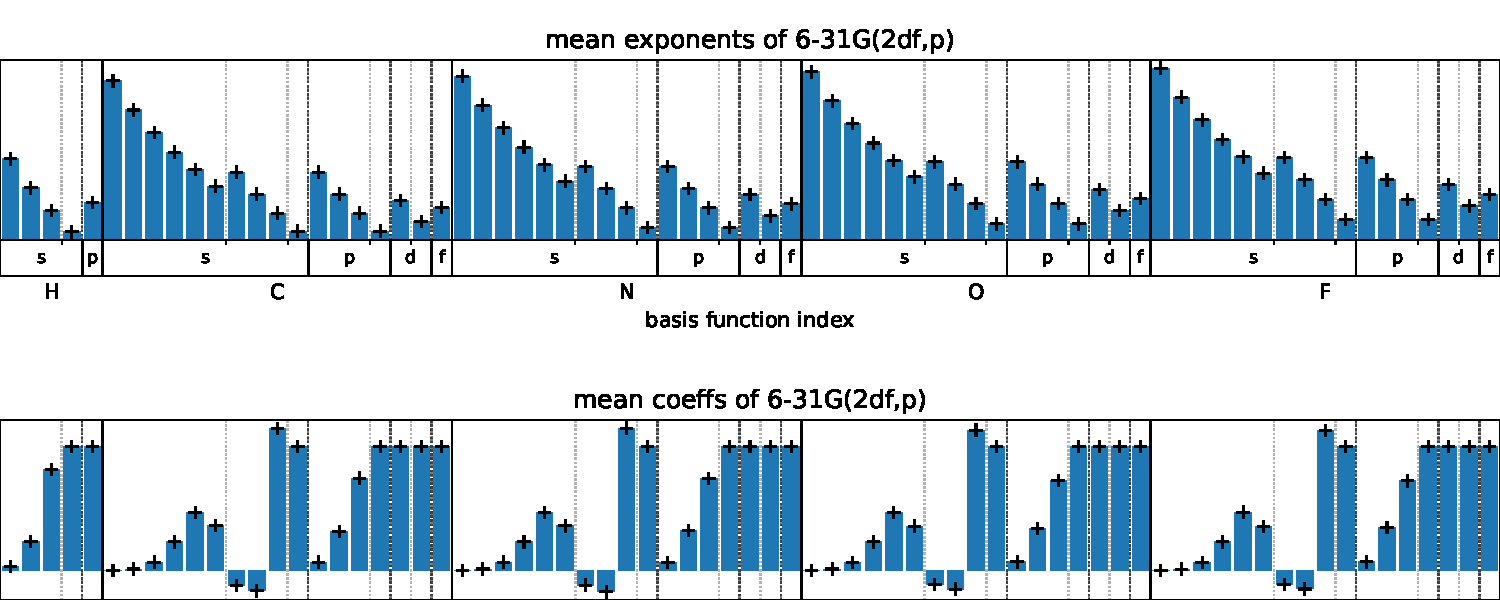
\includegraphics[width=0.75\textwidth]{chapters/results/results_images/adaptive_basis_functions/mean_exps_and_coeffs6-31G(2df,p)}
    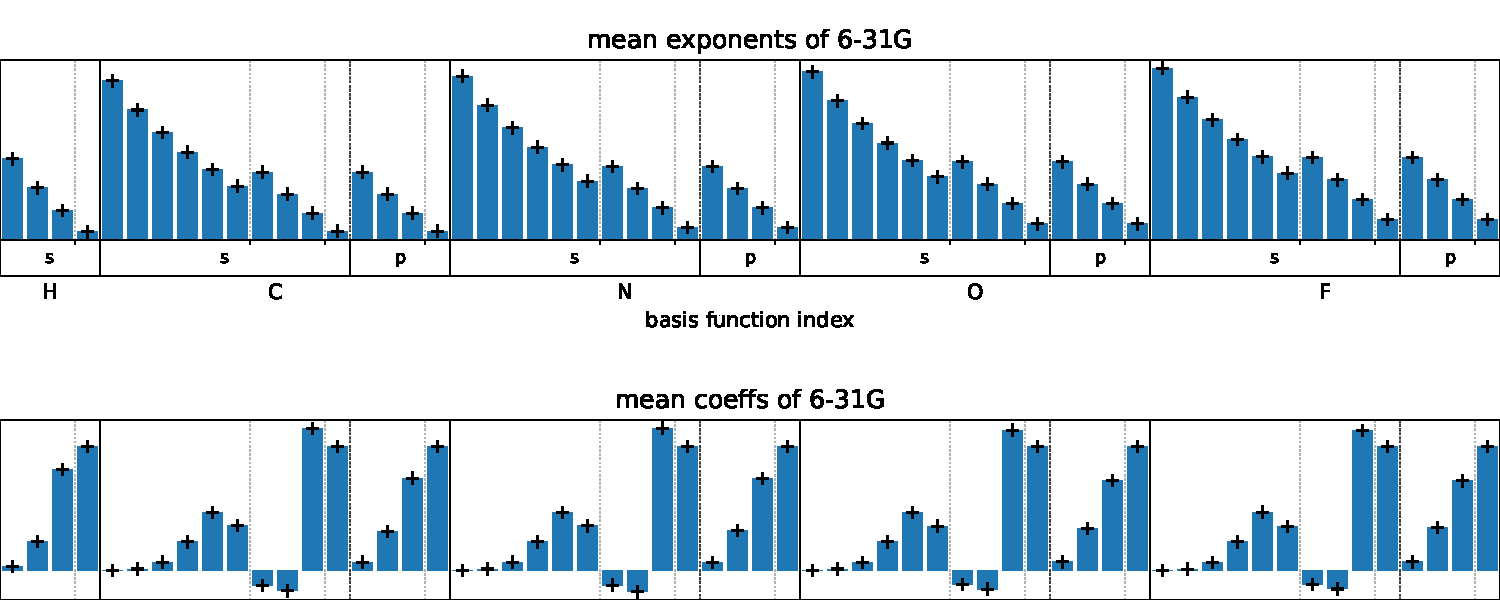
\includegraphics[width=0.75\textwidth]{chapters/results/results_images/adaptive_basis_functions/mean_exps_and_coeffs6-31G}
    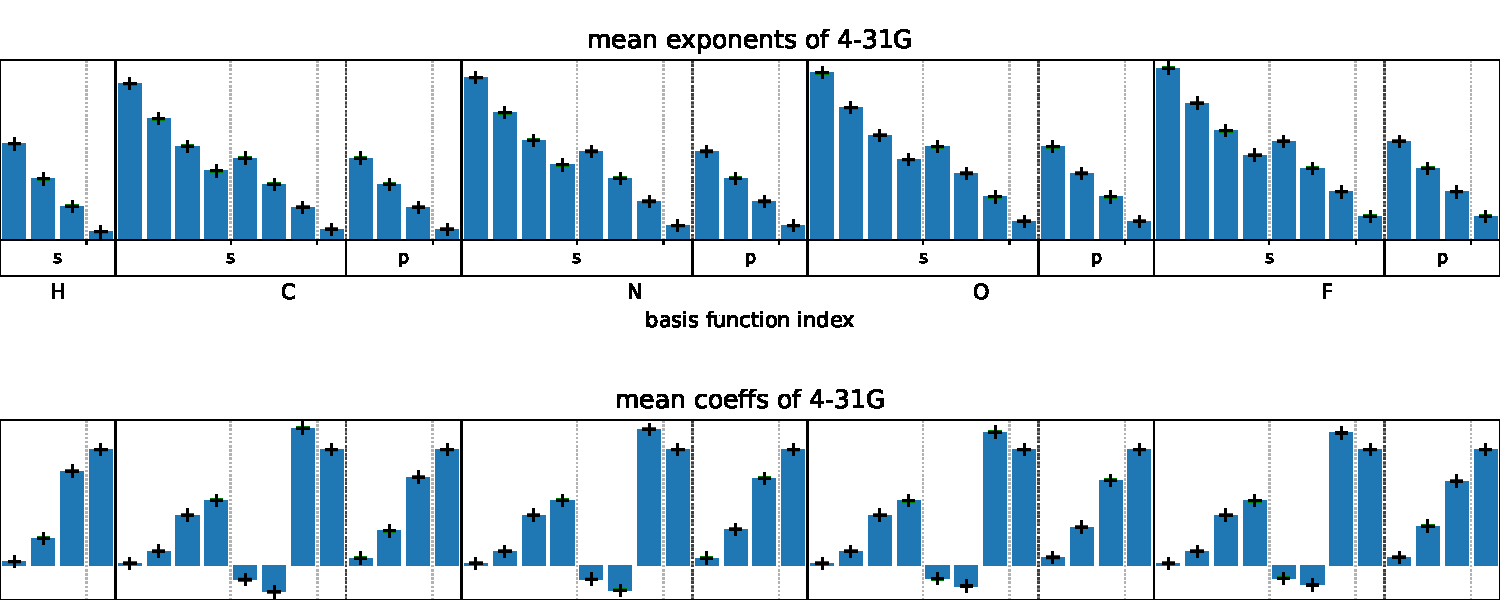
\includegraphics[width=0.75\textwidth]{chapters/results/results_images/adaptive_basis_functions/mean_exps_and_coeffs4-31G}
    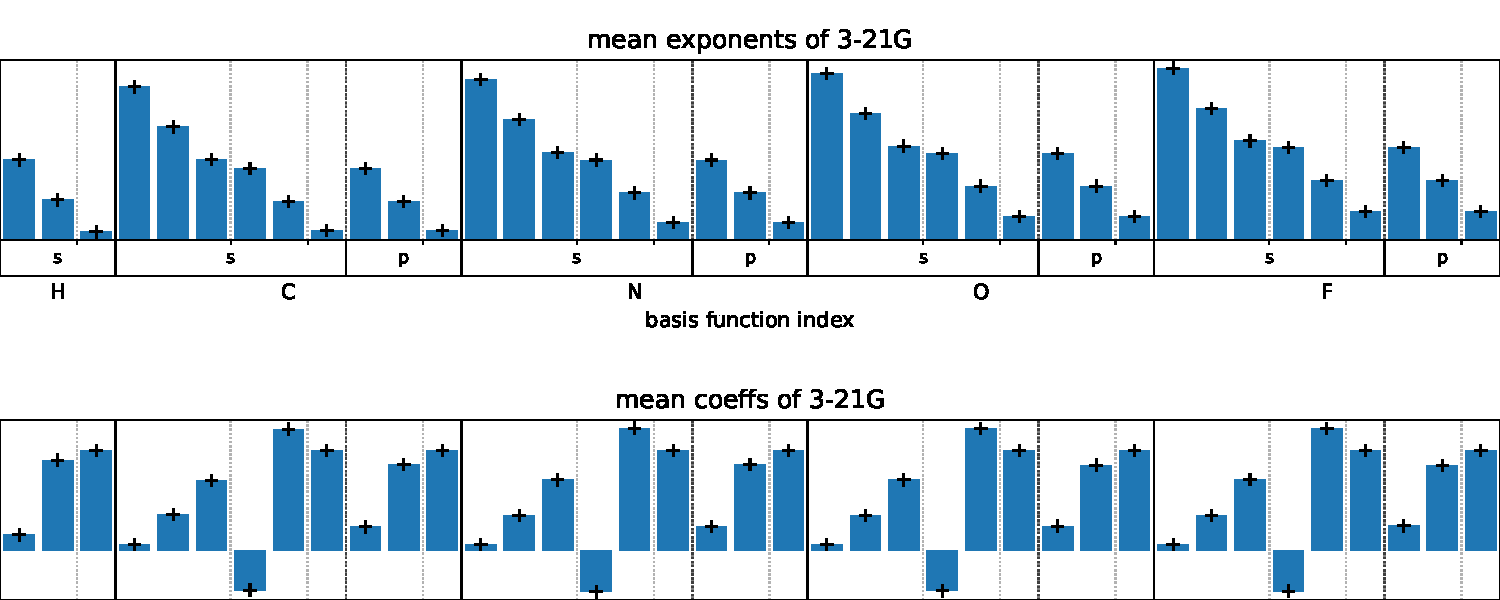
\includegraphics[width=0.75\textwidth]{chapters/results/results_images/adaptive_basis_functions/mean_exps_and_coeffs3-21G}
    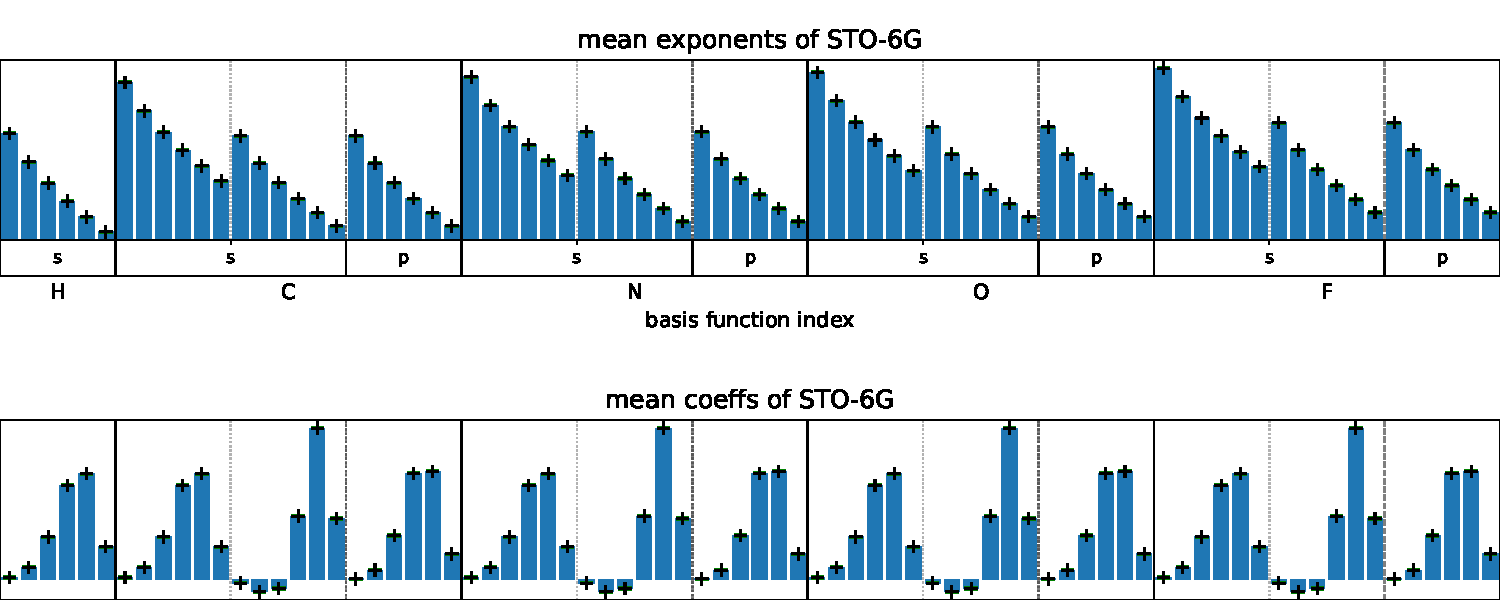
\includegraphics[width=0.75\textwidth]{chapters/results/results_images/adaptive_basis_functions/mean_exps_and_coeffsSTO-6G}
    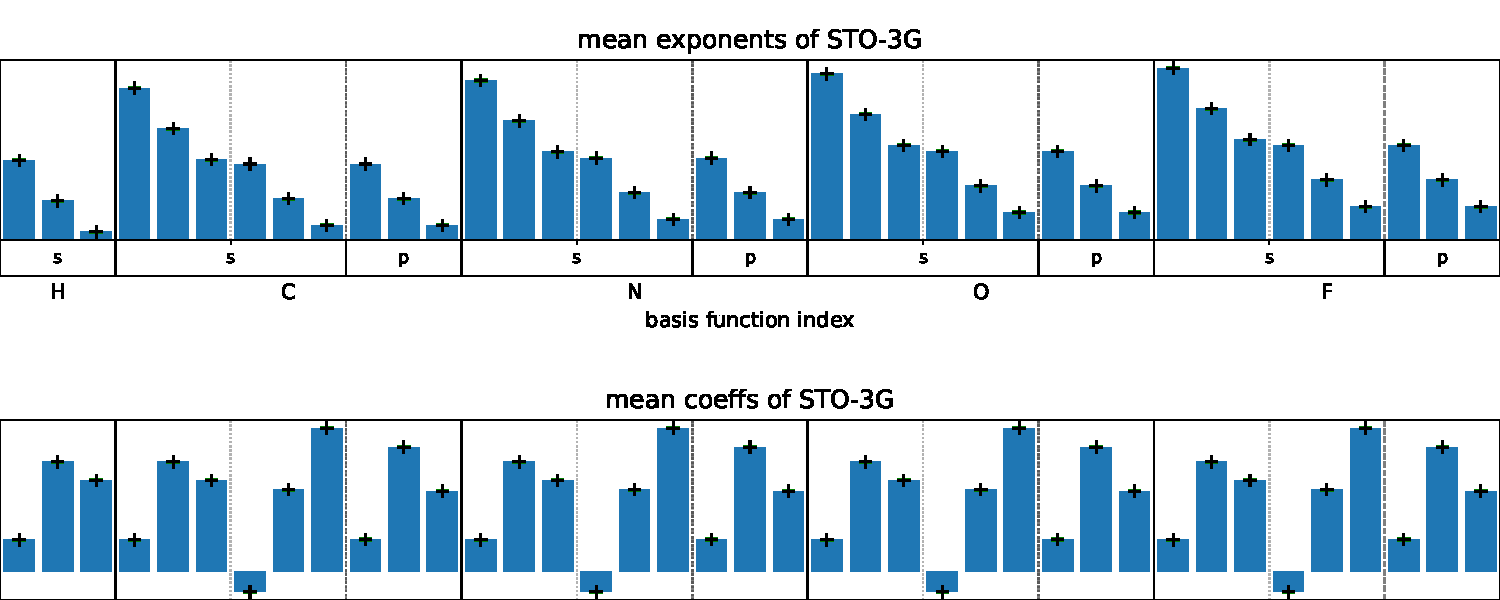
\includegraphics[width=0.75\textwidth]{chapters/results/results_images/adaptive_basis_functions/mean_exps_and_coeffsSTO-3G}
    \caption{Contraction coefficients and exponents of the different classical basis sets. The light dottet lines indicate sets of exponents and coefficints which are contracted into a single basis function. The thicker dotted lines seperate different shells and the solid lines seperate different atomtypes. The corresponding coeff. for each exponent is plotted directly below it.} \label{fig:classical_exps_coeffs}
\end{figure}

\begin{figure}
    \centering
    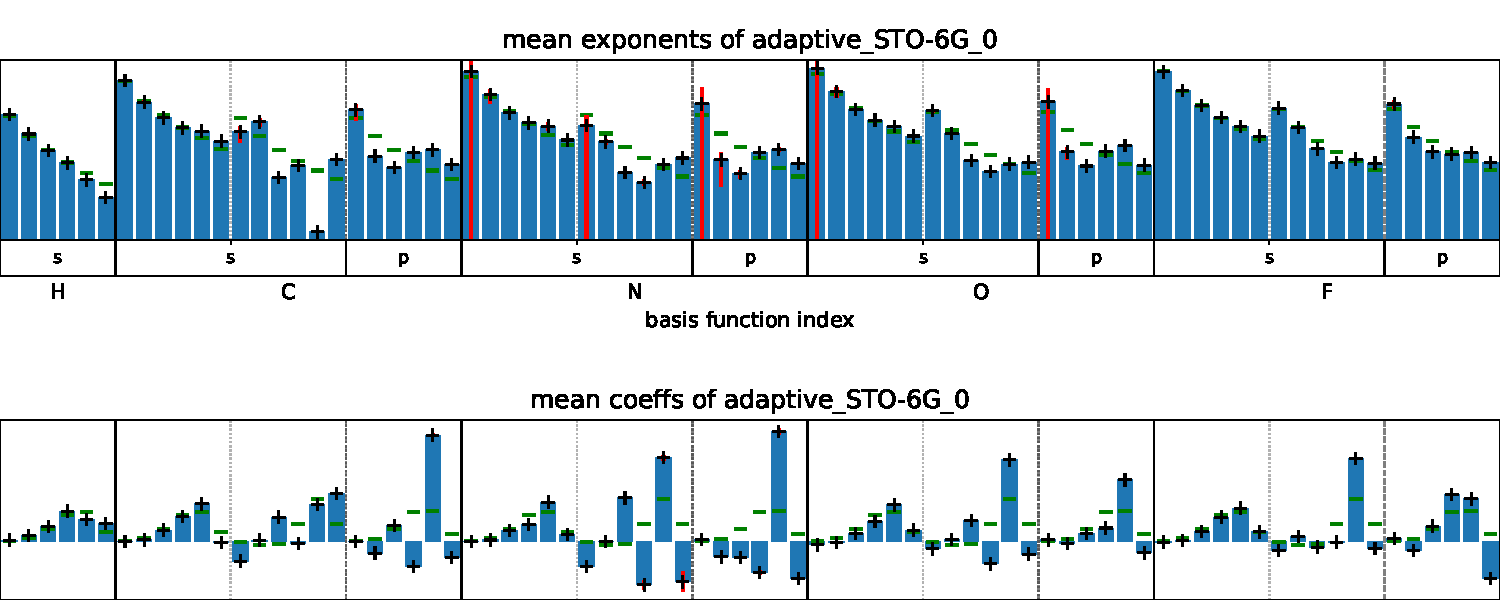
\includegraphics[width=0.75\textwidth]{chapters/results/results_images/adaptive_basis_functions/mean_exps_and_coeffsadaptive_STO-6G_0}
    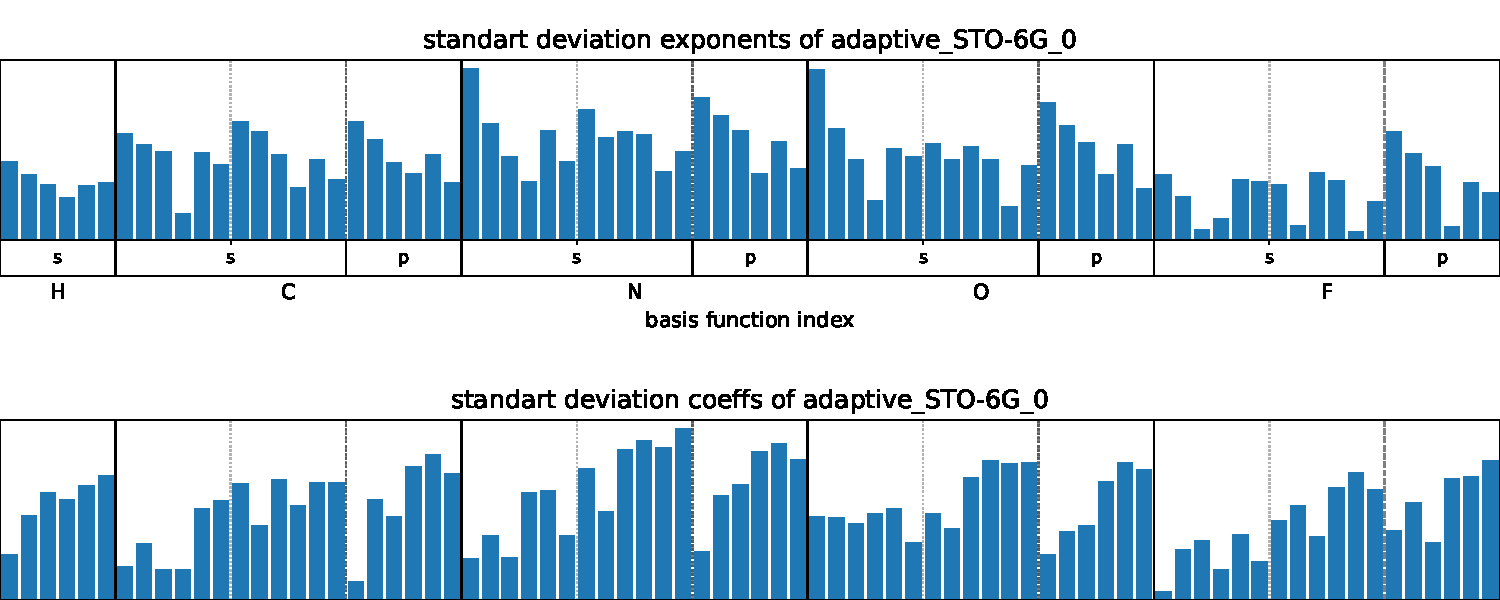
\includegraphics[width=0.75\textwidth]{chapters/results/results_images/adaptive_basis_functions/std_exps_and_coeffsadaptive_STO-6G_0}
    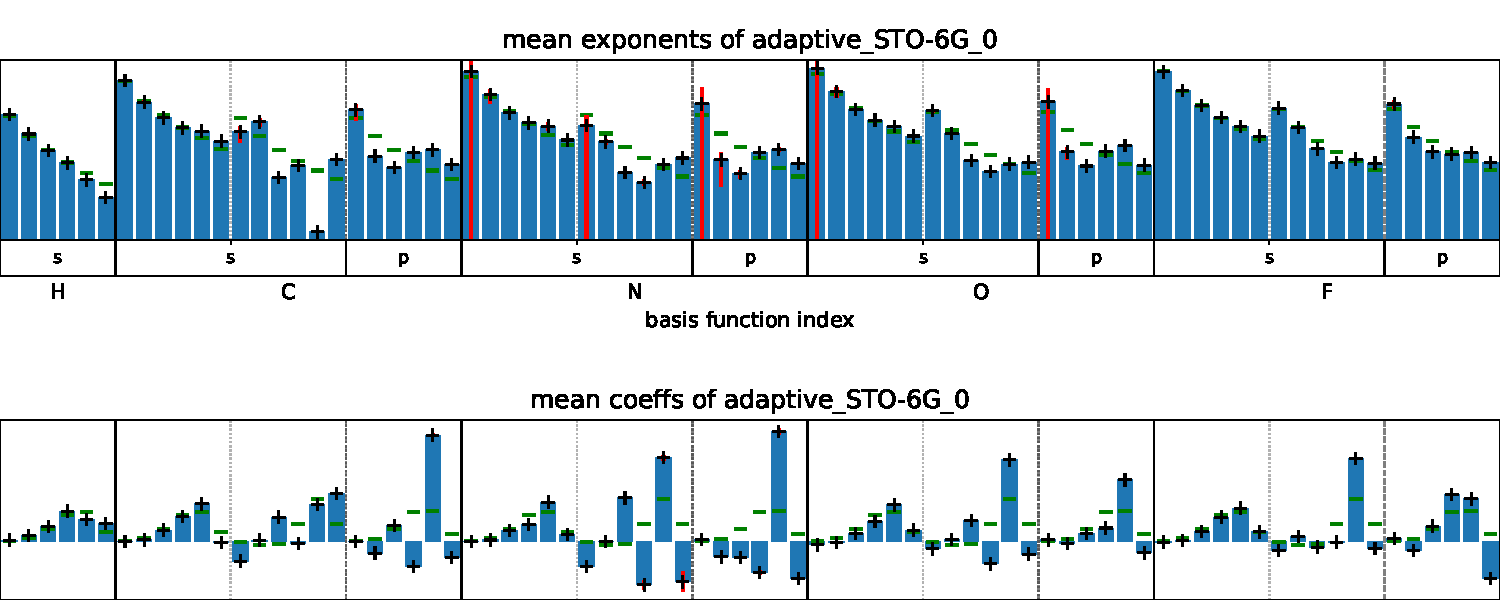
\includegraphics[width=0.75\textwidth]{chapters/results/results_images/adaptive_basis_functions/mean_exps_and_coeffsadaptive_STO-6G_0}
    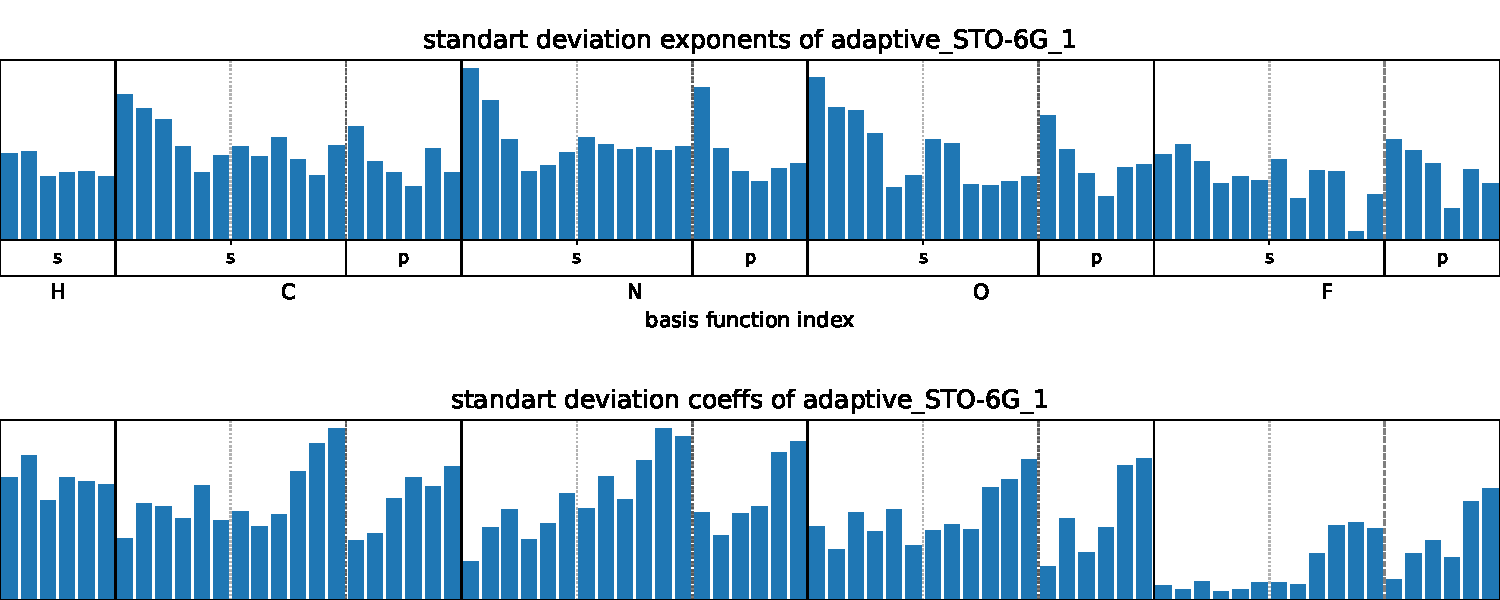
\includegraphics[width=0.75\textwidth]{chapters/results/results_images/adaptive_basis_functions/std_exps_and_coeffsadaptive_STO-6G_1}
\end{figure}

\begin{figure}
    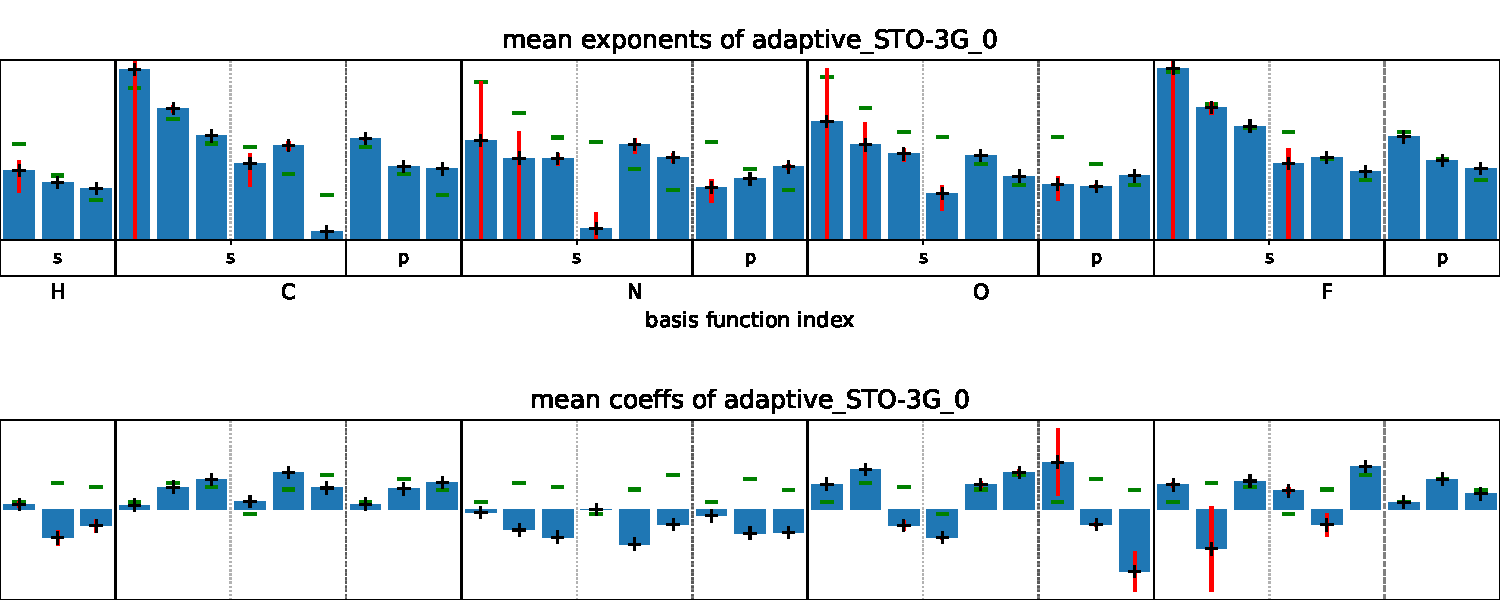
\includegraphics[width=0.75\textwidth]{chapters/results/results_images/adaptive_basis_functions/mean_exps_and_coeffsadaptive_STO-3G_0}
    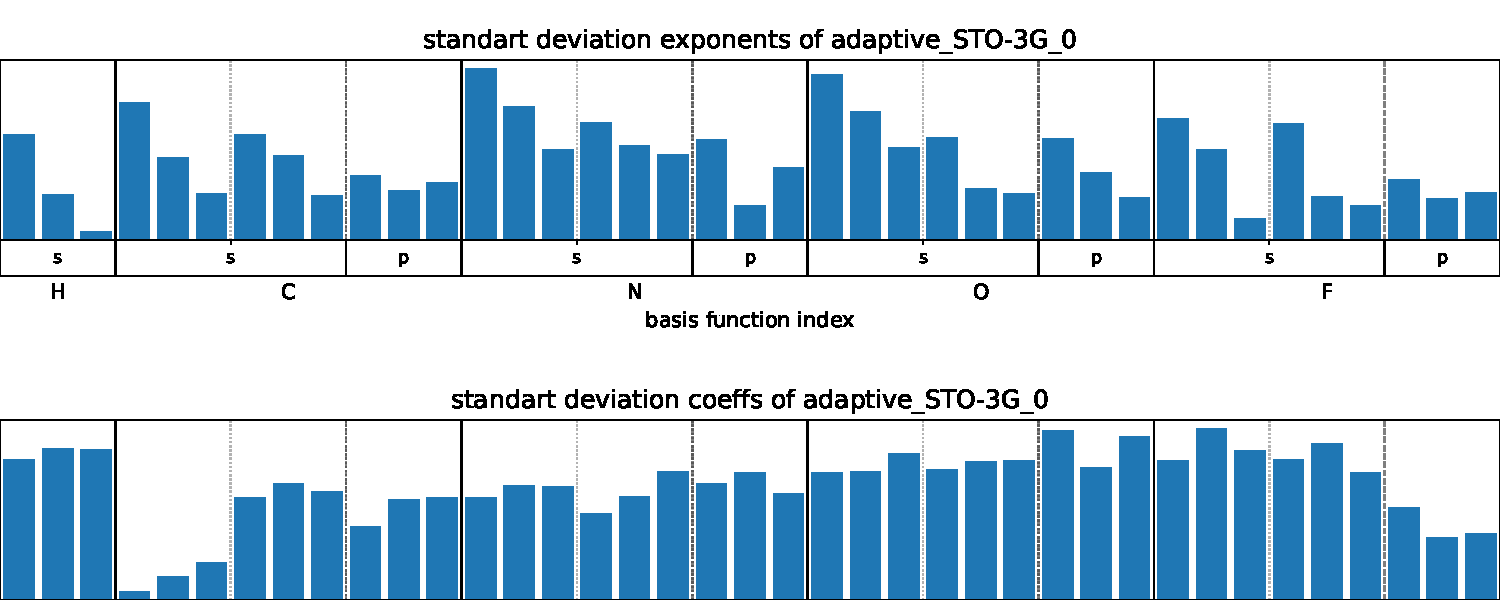
\includegraphics[width=0.75\textwidth]{chapters/results/results_images/adaptive_basis_functions/std_exps_and_coeffsadaptive_STO-3G_0}
    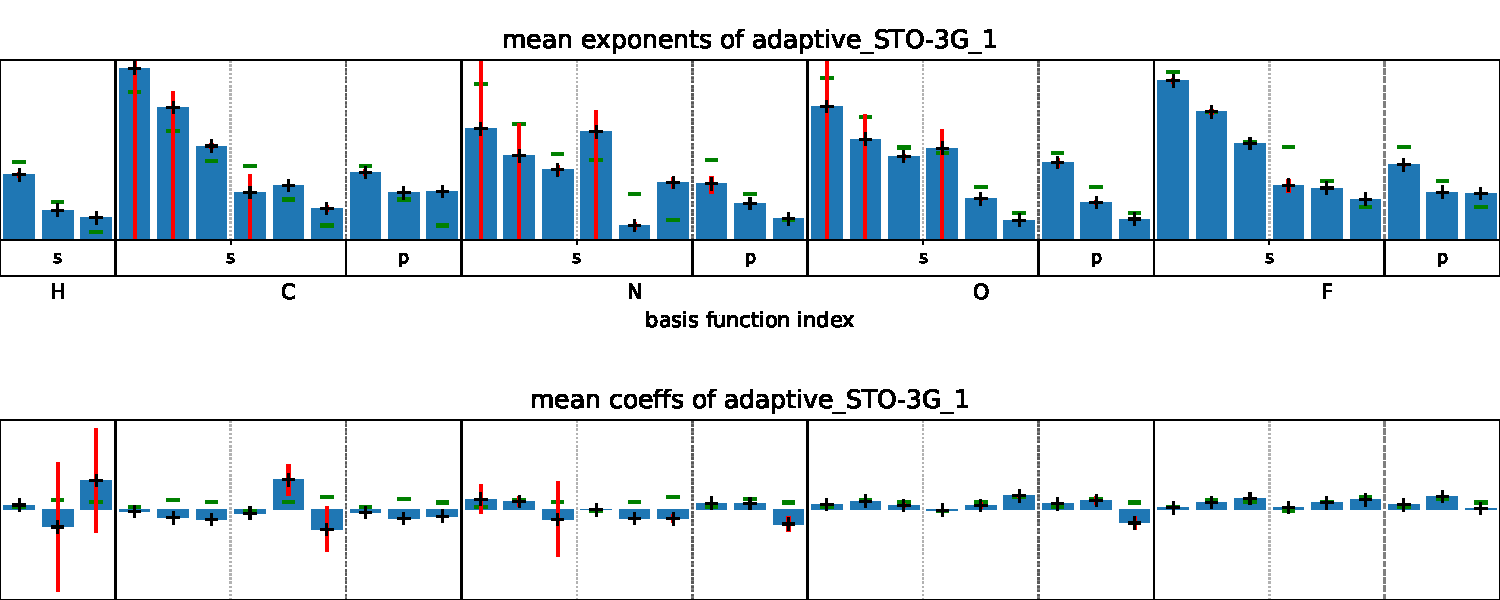
\includegraphics[width=0.75\textwidth]{chapters/results/results_images/adaptive_basis_functions/mean_exps_and_coeffsadaptive_STO-3G_1}
    \end{figure}

\begin{figure}
    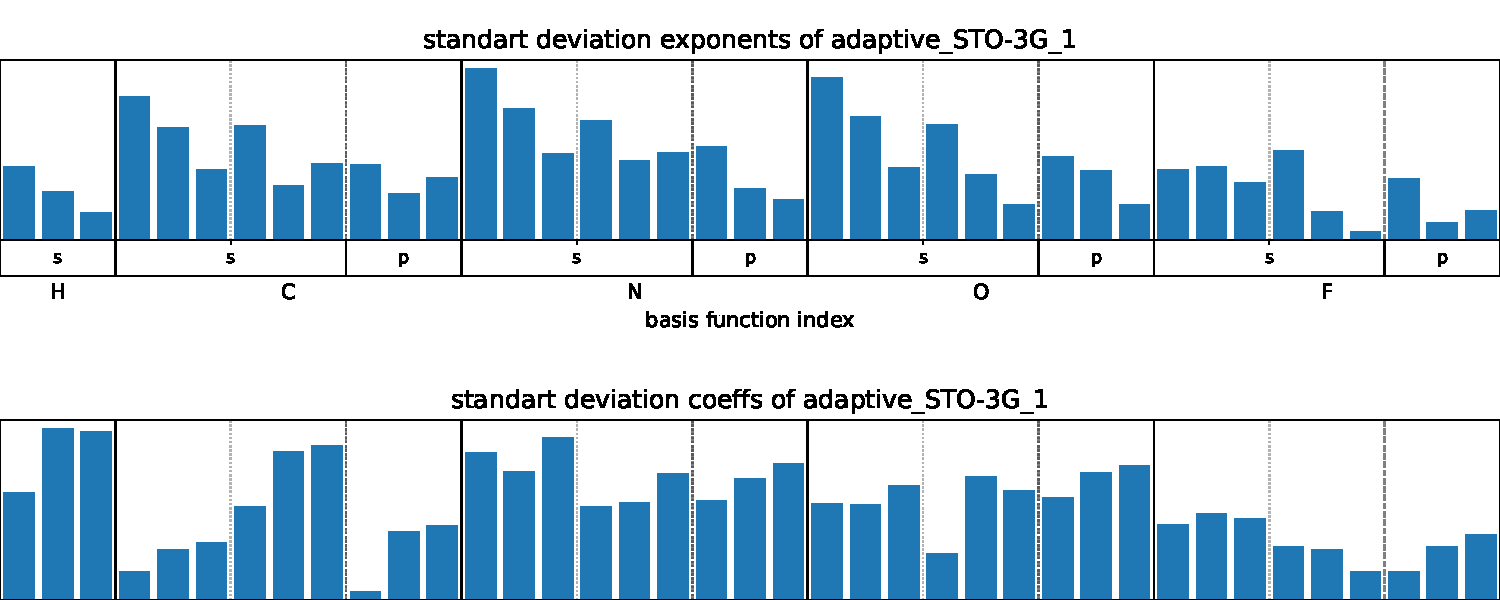
\includegraphics[width=0.75\textwidth]{chapters/results/results_images/adaptive_basis_functions/std_exps_and_coeffsadaptive_STO-3G_1}
    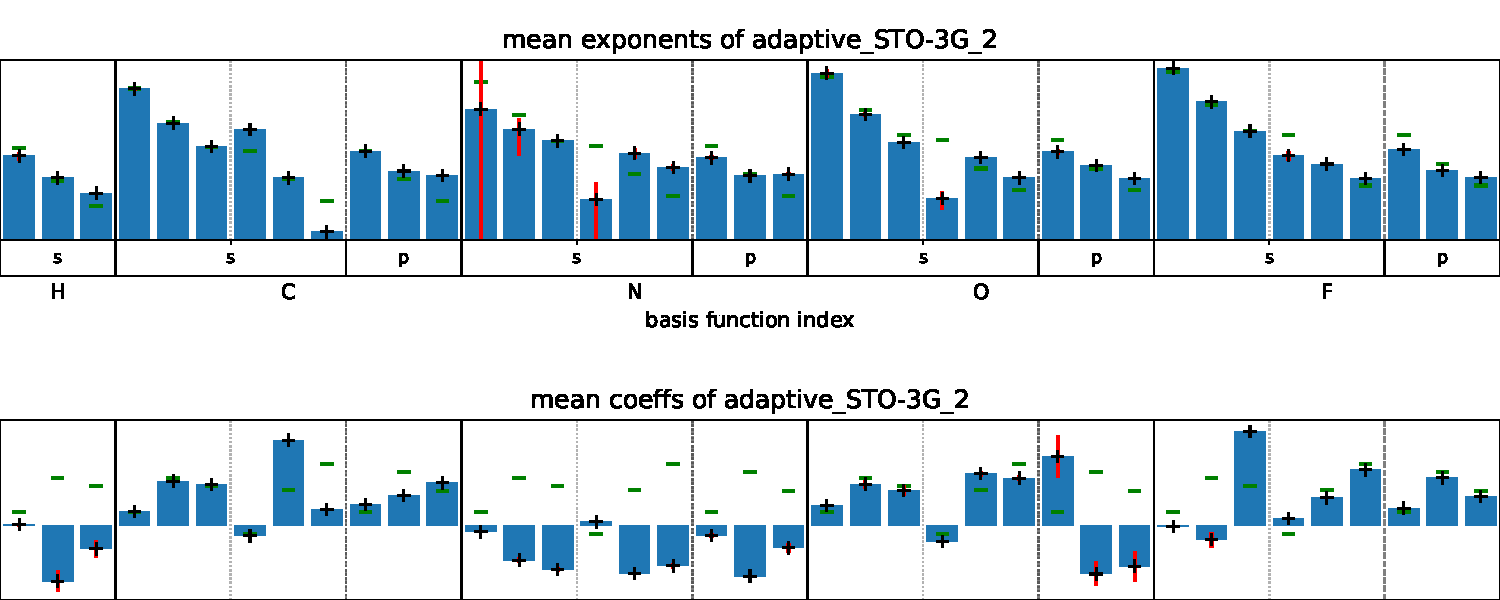
\includegraphics[width=0.75\textwidth]{chapters/results/results_images/adaptive_basis_functions/mean_exps_and_coeffsadaptive_STO-3G_2}
    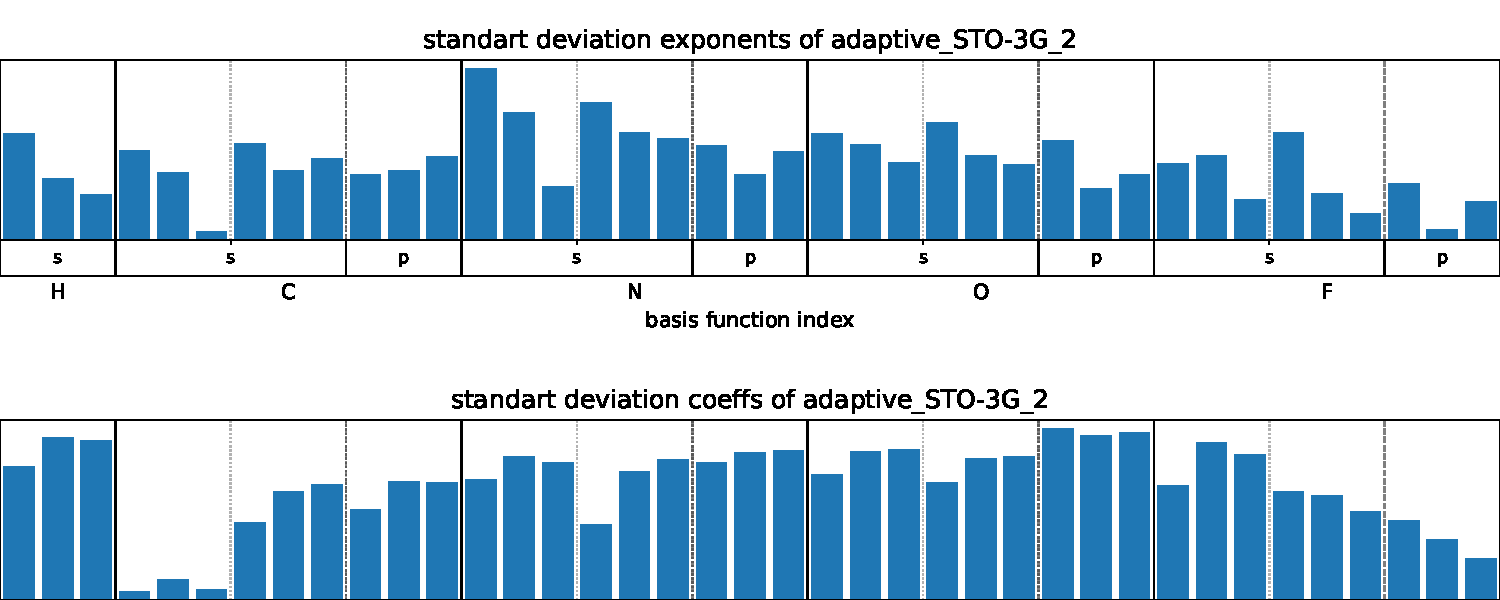
\includegraphics[width=0.75\textwidth]{chapters/results/results_images/adaptive_basis_functions/std_exps_and_coeffsadaptive_STO-3G_2}
    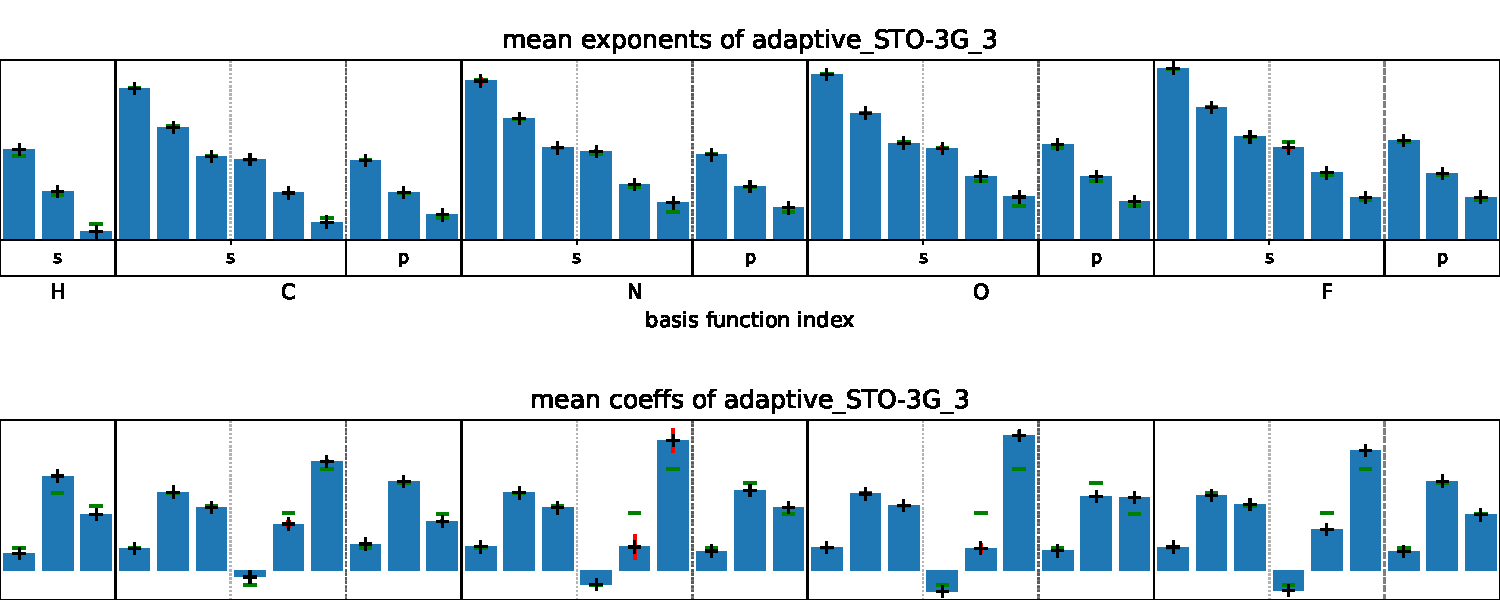
\includegraphics[width=0.75\textwidth]{chapters/results/results_images/adaptive_basis_functions/mean_exps_and_coeffsadaptive_STO-3G_3}
    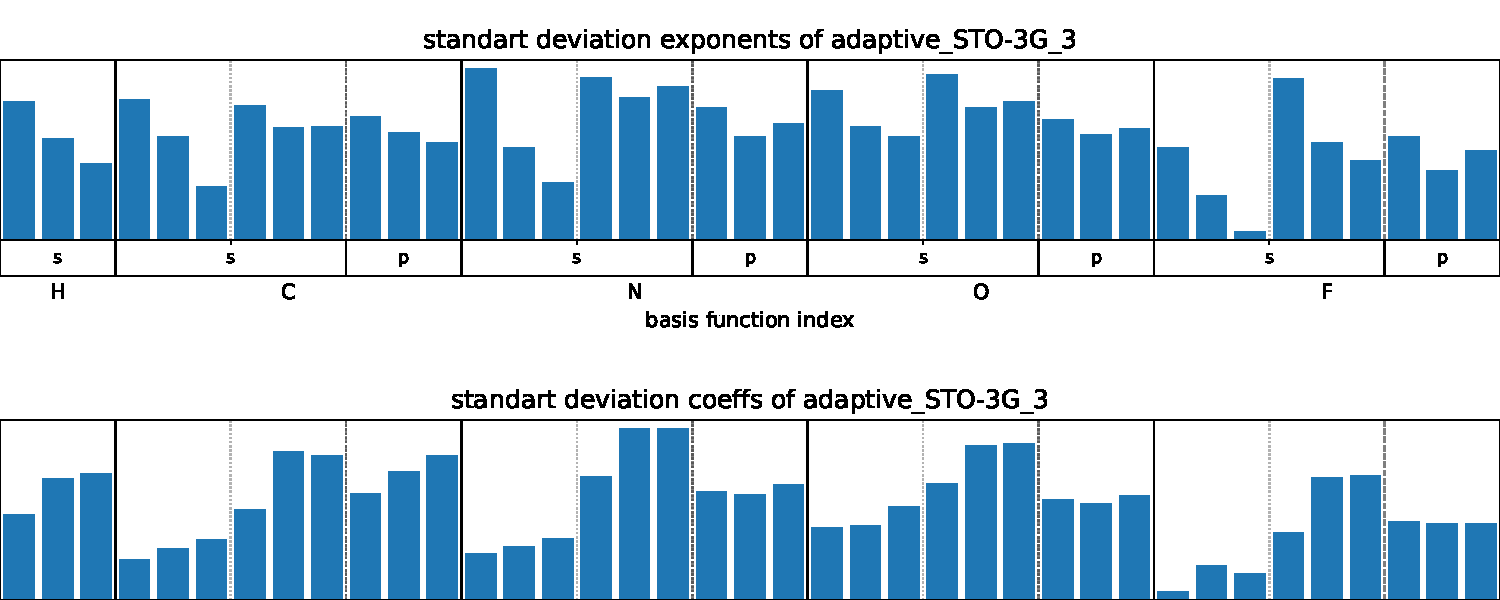
\includegraphics[width=0.75\textwidth]{chapters/results/results_images/adaptive_basis_functions/std_exps_and_coeffsadaptive_STO-3G_3}
\end{figure}






